\subsection{SRGAN}


Las CNN presentan un gran avance en la reconstrucción de imágenes de baja resolución a alta resolución,
sin embargo, debido a los metodos basados en interpolaciónes 


Las GAN´s (Generative Adversarial Networks) son un tipo de redes cuyo funcionamiento está basado
en la estimación de modelos generadores, como mencionan Goodfellow et al. \cite{GANs}, esto es 
posible gracias al entrenamiento simultáneo de dos modelos, uno \emph{generador (G)} que obtiene 
la distribución de la entrada para generar datos falsos y el otro \emph{discriminador (D)} el cual se encarga de estimar 
la probabilidad de que la muestra provenga del dataset de entrenamiento y discernir así entre estos datos y 
los del modelo \emph{ generador (G)}.

El término \emph{antagónicas} como se menciona en \cite{SRGAN_Tesis}, se refiere a la dinámica 
competitiva que se mantiene entre los dos modelos. Por un lado,
el generador tiene por objetivo crear nuevos datos que sean indistinguibles del
conjunto de entrenamiento, mientras que el discriminador debe poder ser capaz
de distinguir cuáles son los datos creados y los reales, siendo los últimos los que corresponden
 al conjunto de entrenamiento. Esto resulta en un proceso iterativo donde estos dos modelos
 se desafían uno a otro, logrando un ajuste de parámetros
 que logran producir datos que se parezcan con gran acierto a los reales.
 

\begin{figure}[H]
    \begin{center}
      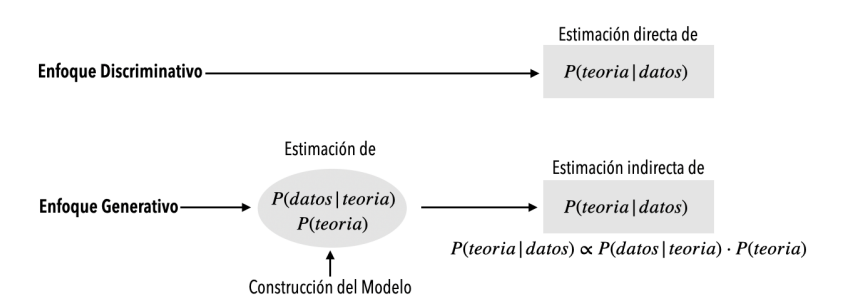
\includegraphics[scale = 0.9]{modelo_gen_disc.png}
      \caption{Modelo Generador y Discriminador}
      \label{Alex1}
    \end{center}
    \end{figure}